% vim: set spelllang=fr foldmethod=marker:
\section{Résultats numériques}
\label{sa:sec:resultats}
%===============================================================================
    \subsection{Modèle de la simulation}\label{sa:ssec:modelsim}

Afin d'étudier les avantages concrets qu'apporte l'élection dynamique des \cns, nous avons réalisé une série de simulations à l'aide du logiciel \nsii~\cite{ns2}.
Les résultats obtenus sont présentés dans cette section.
Ils sont issus de tests simulant le comportement d'un cluster qui se présente sous la forme d'une grille régulière de dix nœuds de côté par dix (voir \figref{sa:fig:grille}).
Nous supposons, lorsque la question se pose, que c'est le protocole \leach qui a été mis en œuvre pour établir ce cluster.
\begin{figure}[!b]
    \centering
    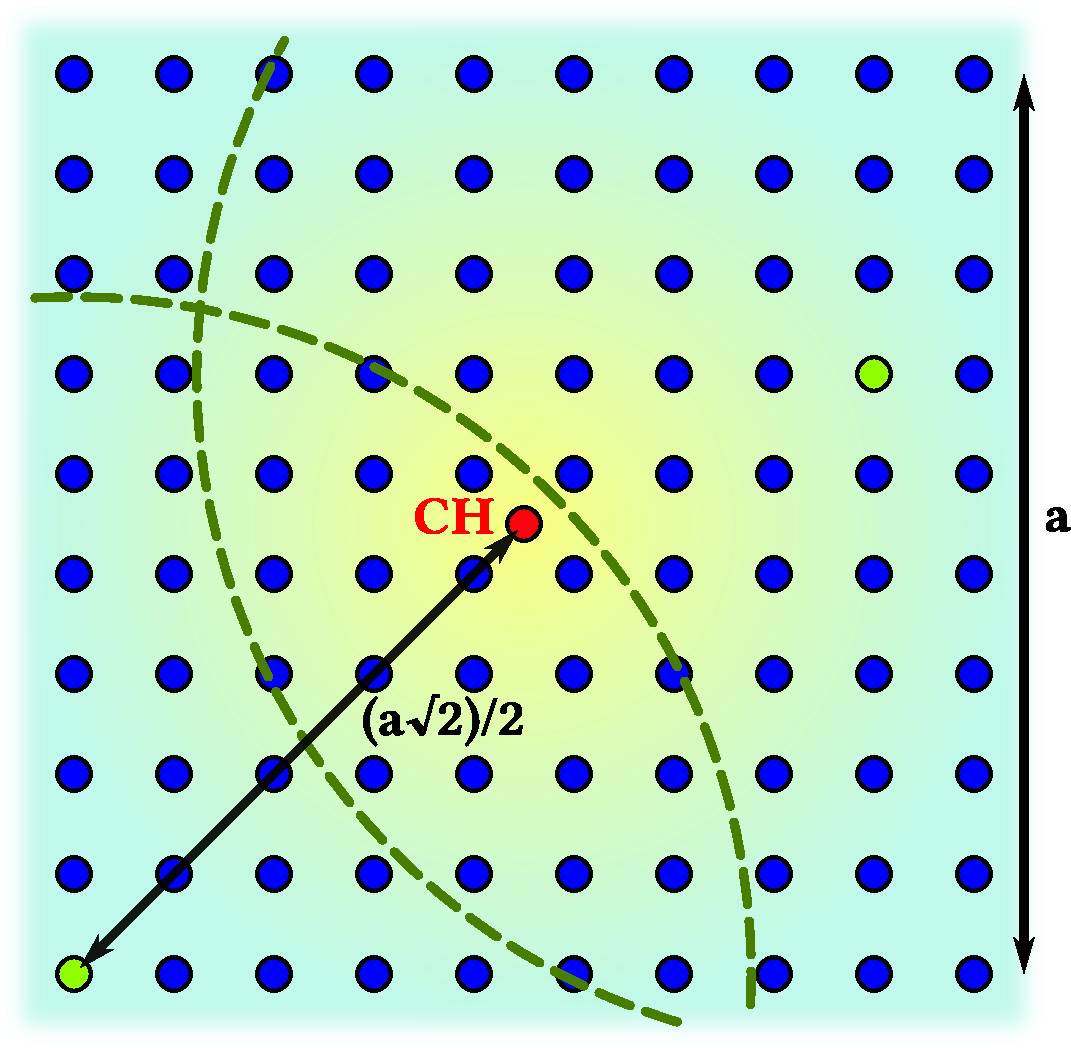
\includegraphics[width=6.5cm]{\chapterfig/WSN_topo.pdf}
    \caption{Cluster sous forme de grille régulière $10 \times 10$, de côté de longueur $a$}\label{sa:fig:grille}
\end{figure}

Les caractéristiques du cluster étudié sont les suivantes:
\begin{itemize}
    \item la grille est un carré de côté de longueur $a$;
    \item le \ch est placé au centre géométrique de la grille;
    \item la grille contient cent capteurs, disposés régulièrement à chaque nœud de la grille;
    \item chaque capteur peut communiquer directement avec le \ch; autrement dit, chaque nœud a une portée au moins équivalente à la distance $\frac{a \sqrt{2}}{2}$, soit une sphère de rayon égal à la moitié de la diagonale du carré. Chaque capteur, y compris ceux situés dans les coins du carré, peut ainsi communiquer avec le \ch sans intermédiaire. Aucun ajustement de la puissance de transmission n'est effectué par les capteurs;
    \item les \cns sont élus selon la méthode statique (unique sélection en début de simulation) ou bien dynamique (élection renouvelée périodiquement), selon le cas.
\end{itemize}

%===============================================================================
    \subsection{Taux de détection des nœuds compromis}\label{sa:ssec:detec}

Pour mesurer l'efficacité des \cns, nous avons effectué plusieurs tests avec \nsii.
La \tabref{sa:table:parametres1} indique les valeurs (ou les fourchettes de valeurs) utilisées comme paramètres au cours des différentes simulations.
\begin{table}[ht]
    \centering
    \caption{Paramètres de simulation}\label{sa:table:parametres1}
    \medskip
    \begin{tabular}{lc}
        \toprule
        \textsc{Paramètre}        & \textsc{Valeur}\\
        \midrule
        Durée de la simulation    & 100--3\,600~s\\
        Taux d'émission           & 10--800~kbits/s\\
        Taille des paquets        & 500--800~octets\\
        Nombre de nœuds           & 100 (+~\ch)\\
        Nombre de \cns            & 0--30\\
        Nombre de nœuds compromis & 1\\
        \bottomrule
    \end{tabular}
\end{table}

Pour la première simulation, les nœuds sont élus de façon dynamique sur dix périodes consécutives.
Nous avons supposé que la génération de trafic suit une loi de \textsc{Poisson} (la génération est aléatoire, mais l'on connait sa valeur moyenne).
On nomme $\lambda_i$ le paramètre de cette loi appliquée au nœud $i$ (et $\lambda_c$ est le nombre moyen de messages envoyés par seconde par le nœud compromis).
La \figref{sa:fig:detec-nbcn} présente le taux de détection du nœud compromis pour différentes quantités de \cns dans le réseau, par période.
Au cours de la seconde période de la simulation impliquant dix \cns, nous obervons qu'aucun \cn n'a détecté le nœud compromis: les \cns n'étaient donc pas répartis efficacement dans le cluster.
Lorsque leur nombre monte à quinze, il y a, en moyenne sur les périodes, trois \cns qui détectent le capteur corrompu.
Lorsque ce nombre s'accroit encore, il n'y a plus d'évolution notable.
Quinze \cns semblent donc être une mesure idéale pour notre réseau, si l'on considère une élection statique.
En revanche, on peut très bien descendre à dix \cns si l'on envisage un processus d'élection dynamique: le nœud compromis ne sera peut-être pas détecté sur une période donnée, mais le renouvellement rapide des \cns permet de s'assurer qu'il sera détecté rapidement sur la période suivante.
On note par ailleurs que jusqu'à quarante pour cent (soit quatre nœuds sur dix) ont pu détecter simultanément le nœud compromis sur les périodes~7,~8~et~9.
\begin{figure}[t]
    \centering
    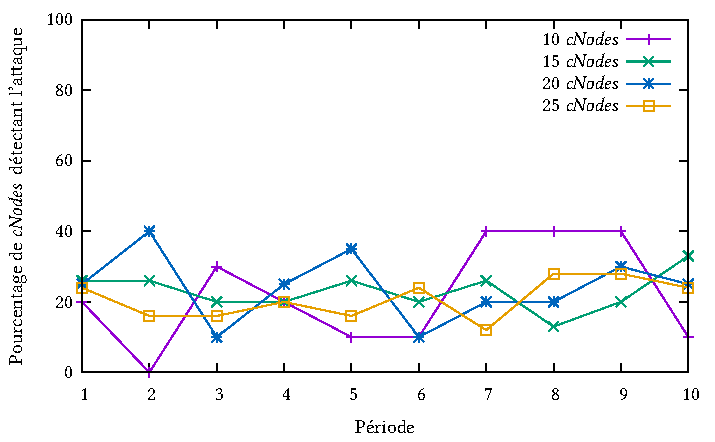
\includegraphics{\chapterfig/plot_detection-nbCNodes.pdf}
    \caption{Taux de détection pour différents nombres de \cns}\label{sa:fig:detec-nbcn}
\end{figure}

La valeur de $\lambda_c$ a elle aussi un rôle à jouer dans la détection: plus le nœud compromis émet, plus il est probable que les \cns mesureront efficacement un dépassement par rapport au seuil théorique d'un nœud honnête.
\begin{figure}[!b]
    \centering
    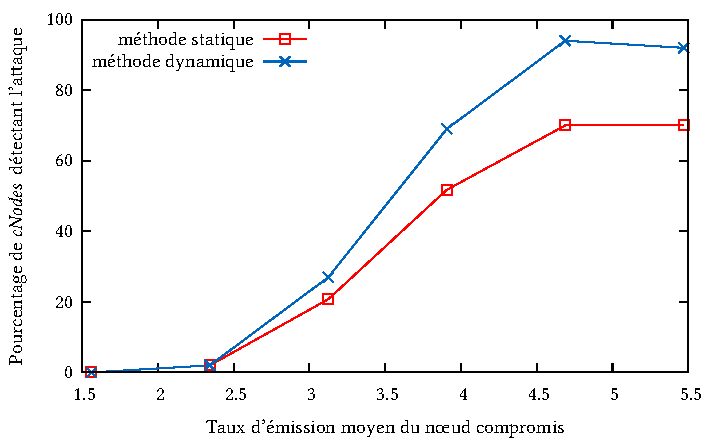
\includegraphics{\chapterfig/plot_detection-txRate.pdf}
    \caption{Taux de détection en fonction de $\lambda_c$}\label{sa:fig:detection-txRate}
\end{figure}
Mais ici encore, le renouvellement rapide des \cns apporte une meilleure détection, puisque statistiquement, davantage de voisins proches du nœud compromis se retrouveront \cns à un moment ou l'autre au cours de la simulation.
La courbe présentée en \figref{sa:fig:detection-txRate} illustre cet état de fait.

%===============================================================================
    \subsection{Consommation énergétique}

Les paramètres utilisés pour les simulations présentées dans cette sous-section sont synthétisés en \tabref{sa:table:parametres2}.
\begin{table}[ht]
    \centering
    \caption{Paramètres de simulation}\label{sa:table:parametres2}
    \medskip
    \begin{tabular}{lc}
        \toprule
        \textsc{Paramètre}                    & \textsc{Valeur}\\
        \midrule
        Durée de la simulation                & 500~secondes\\
        Nombre de capteurs                    & 100\\
        Consommation énergétique en réception & 0,394~W\\
        Consommation énergétique en émission  & 0,660~W\\
        \bottomrule
    \end{tabular}
\end{table}

L'histogramme donné en \figref{sa:fig:conso-moyenne} expose la consommation en énergie des nœuds, pour la méthode d'élection statique et pour la méthode dynamique, en fonction du pourcentage de \cns.
\begin{figure}[!b]
    \centering
    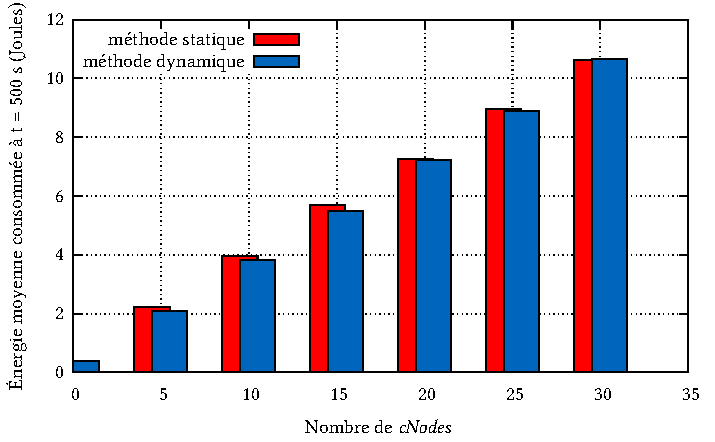
\includegraphics{\chapterfig/plot_mean.pdf}
    \caption{Consommation moyenne en énergie}\label{sa:fig:conso-moyenne}
\end{figure}
Par «consommation en énergie», on entend ici la consommation moyenne en fin de simulation ramenée sur la totalité des nœuds, à l'exception du \ch ainsi que du nœud compromis, qui consomment évidemment plus que les autres, et dont le comportement est invariant entre les méthodes statiques et dynamiques.
Pour rappel, les nœuds normaux (non \cns) ne reçoivent pas les messages de leurs voisins et donc ne consomment pas d'énergie en dehors de leur période d'émission (voir le fonctionnement détaillé de \leach au \chapref{st}, \sssref{st:subsubsec:leach}).
La consommation moyenne en fin de simulation est identique pour les deux méthodes: il s'agit d'un résultat attendu, puisque les deux méthodes mettent en œuvre, à tout instant $t$, autant de nœuds normaux et de \cns l'une que l'autre.

En revanche, si l'on compare les écarts-types à la moyenne, on relève des différences notables.
Elles sont manifestes sur l'histogramme présenté en \figref{sa:fig:conso-ecart-type}, qui présente, pour différents pourcentages de \cns, les écarts-types à la moyenne précédente de la consommation en énergie des nœuds, à la fin de la simulation.
Ici encore, \ch et nœud compromis ont été laissés de côté.
Nous observons des écarts-types bien plus forts pour la méthode statique: seuls les \cns initiaux (non soumis à réélection par la suite) ont connu une consommation importante ---~ils sont restés sur écoute, ont analysé le trafic, éventuellement averti le \ch d'une attaque.
Avec la méthode dynamique cependant, les écarts de consommations sont lissés sur le temps du fait des réélections périodiques.
Nous observons ainsi une meilleure répartition de la charge.
\begin{figure}[ht]
    \centering
    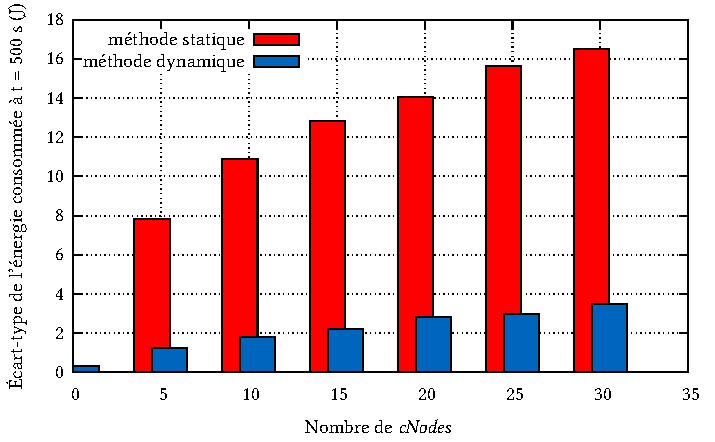
\includegraphics{\chapterfig/plot_stddev.pdf}
    \caption{Écart-type à la moyenne de la consommation en énergie}\label{sa:fig:conso-ecart-type}
\end{figure}

L'histogramme de la \figref{sa:fig:premier-deces} présente l'instant de décès du premier nœud à épuiser sa batterie au sein du cluster simulé.
Pour obtenir ce résultat, nous avons alloué une énergie initiale de 4~\joule à chacun des nœuds (excepté le nœud compromis et le \ch, qui ont reçu davantage d'énergie, car nous ne voulions pas qu'ils cessent de fonctionner durant la simulation).
À noter: la valeur de 4~\joule initialement allouée aux nœuds est une valeur très faible.
Mais de même, cinq-cents secondes de simulation sont très courtes au regard de la durée de vie réelle d'un capteur.
Une pile au lithium (de modèle CR~1225 par exemple) offre environ 540~\joule; une pile~AA (ou~LR06) fournit quant à elle environ 15\,400~\joule, et une pile~AAA (ou~LR03) environ 6\,800~\joule.
À titre d'exemple, plusieurs modèles de capteurs utilisent un couple de piles AAA.
\begin{figure}[ht]
    \centering
    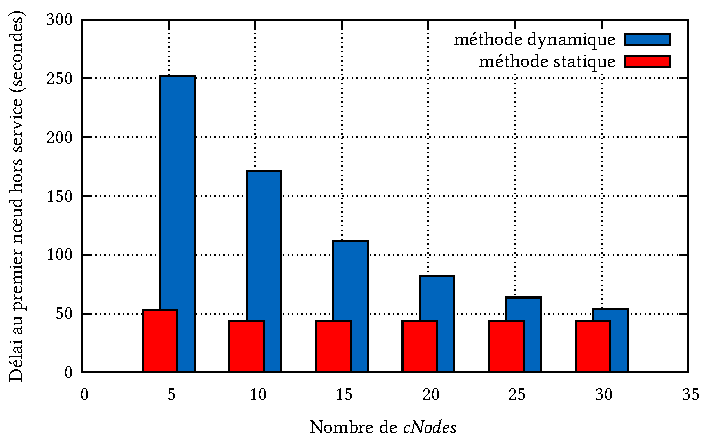
\includegraphics{\chapterfig/plot_fstdth.pdf}
    \caption{Instant de premier décès dans le réseau}\label{sa:fig:premier-deces}
\end{figure}
%
% 1 J = 1 W.s = 1 U*I*t (= V.A.s) = 3600 V.A.h
% LR06: 2850 mAh, 1,5 V --> 3600 * 1,5 * 2,850 = 15390 J ~ 15400 J
% LR03: 1250 mAh, 1,5 V --> 3600 * 1,5 * 1,250 = 6750 J ~ 6800 J
% CR1225: 50 mAh, 3 V --> 3600 * 3 * 0,050 = 540 J

C'est donc avec 4~\joule en réserve qu'ont démarré les capteurs, de sorte que l'on puisse effectivement observer les pannes.
Nous avons démarré la simulation, et relevé l'instant de «décès» du premier nœud vidé de ses réserves d'énergie.
En raison du changement périodique de \cns, la méthode dynamique permet de mieux répartir la consommation en énergie, là où la méthode statique sollicite toujours les mêmes \cns.
Le premier nœud à épuiser sa batterie a donc une espérance de vie bien plus longue avec la méthode dynamique (jusqu'à cinq fois plus longue lorsque le pourcentage de \cns est faible), comme le reflète l'histogramme.

%===============================================================================
    \subsection{Nœuds restants et détection au fil du temps}

Au cours de cette dernière simulation, nous avons observé le nombre de nœuds toujours «en vie», ainsi que le nombre de nœuds détectant le nœud compromis au cours du temps.
La durée de la simulation a été étendue à une heure, et les nœuds se sont vus allouer une réserve initiale d'énergie égale à 10~\joule.
Dix pour cent d'entre eux, soit dix à la fois, ont été désignés en tant que \cns.
Ces données, et les autres paramètres utilisés, sont présentés en \tabref{sa:table:parametres3}.
\begin{table}[ht]
    \centering
    \caption{Paramètres de simulation}\label{sa:table:parametres3}
    \medskip
    \begin{tabular}{lc}
        \toprule
        \textsc{Paramètre}                    & \textsc{Valeur}\\
        \midrule
        Durée de la simulation                & 3\,600~secondes\\
        Nombre de capteurs                    & 100\\
        Pourcentage de \cns                   & 10~\%\\
        Consommation énergétique en réception & 0,394~W\\
        Consommation énergétique en émission  & 0,660~W\\
        Quantité initiale d'énergie           & 10~\joule\\
        \bottomrule
    \end{tabular}
\end{table}

La courbe de la \figref{sa:fig:capteurs-en-vie} montre l'évolution dans le temps du nombre de capteurs en vie.
Comme précédemment, les capteurs normaux consomment très peu par rapport aux \cns, qui vident leur batterie bien plus rapidement.
En conséquence, les dix \cns élus au départ avec la méthode statique consomment leur énergie, et meurent (vers $t=150$~secondes), tandis que les nœuds normaux vivent beaucoup plus longtemps (environ cinq heures selon nos estimations), mais ne sont plus surveillés.
Avec la méthode dynamique, les \cns changent, et le premier nœud à mourir décède bien plus tard que dans le cas précédent.
Il s'agit d'un nœud qui a été élu \cn sur plusieurs périodes ---~mais pas (à la différence de la méthode statique) en continu sur \textit{toutes} les périodes.
Deux nœuds seulement sont tombés à court d'énergie à $t=700$~secondes avec la méthode dynamique.
En revanche, passé ce stade, les autre nœuds vont rapidement dépérir les uns après les autres; il ne reste plus qu'un nœud en vie à la fin de l'heure de simulation (ceci n'est pas visible sur la courbe).
Ce décès «prématuré» des nœuds pour la méthode dynamique est tout à fait normal et prévisible, puisque la réélection de \cns élève continuellement la consommation de nouveaux nœuds; tandis que pour la méthode statique, une fois les \cns décédés, il n'y a plus que des nœuds normaux, qui consomment beaucoup moins d'énergie.
\begin{figure}[ht]
    \centering
    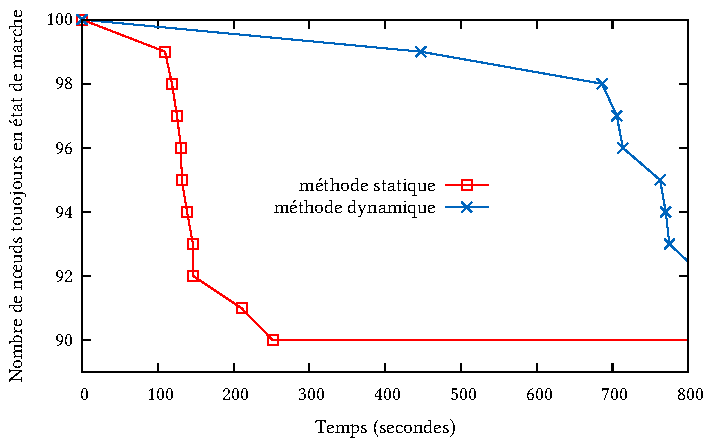
\includegraphics{\chapterfig/plot_lifetime.pdf}
    \caption{Nombre de capteurs toujours en vie}\label{sa:fig:capteurs-en-vie}
\end{figure}

Il est alors intéressant d'observer combien de nœuds sont toujours non seulement en vie, mais aussi capables de détecter l'attaque du nœud compromis au cours du temps.
Les résultats sont exposés par la courbe donnée en \figref{sa:fig:detection-dos}.
Le nombre de \cns ayant détecté l'attaque est indiqué sur chaque période de soixante secondes.
\begin{figure}[ht]
    \centering
    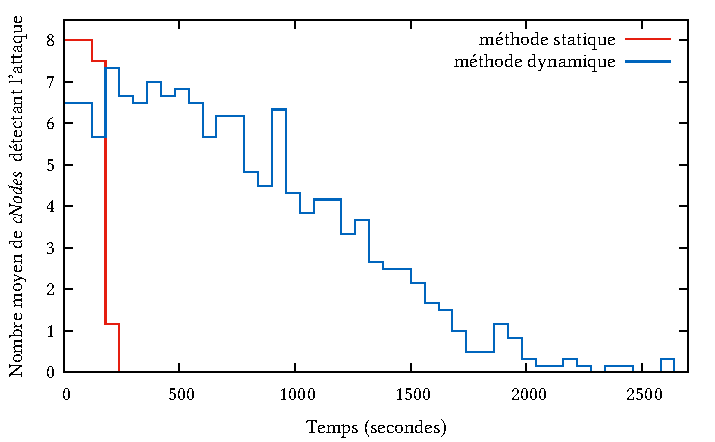
\includegraphics{\chapterfig/plot_dos-over-time.pdf}
    \caption{Détection des attaques de \dds}\label{sa:fig:detection-dos}
\end{figure}
Après la quatrième minute de simulation, tous les \cns élus par la méthode statique ont stoppé leur activité par manque d'énergie, et les attaques ne peuvent plus être détectées.
Avec la méthode dynamique, une moyenne approximative de 6,5~nœuds en vie sur~10 détecte le nœud compromis au cours de chaque période de 60~secondes séparant deux élections.
Le capteur malveillant est toujours détecté par plus d'un nœud en moyenne après une demi-heure de simulation.
